\documentclass[12pt,compress,aspectratio=169]{beamer}

\mode<presentation>
{
  \usetheme{Singapore}
  \setbeamersize{text margin left=1cm,text margin right=1cm}
%  \setbeamertemplate{navigation symbols}{} % suppress nav bar
%  \setbeamercovered{transparent}
}
\usefonttheme{professionalfonts}
\usepackage{amsmath,bm}
\usepackage{siunitx}
%\usepackage{graphicx}
\usepackage{tikz}
\usepackage{mathpazo}
\usepackage[scaled]{helvet}
\usepackage{xcolor,colortbl}
%\usepackage{hyperref}
\usepackage{cancel}

\usetikzlibrary{decorations.pathmorphing,patterns}

\sisetup{
  number-math-rm=\mathnormal,
  per-mode=symbol
}

\title{Topic 7: Universal Gravitation}
\subtitle{Advanced Placement Physics}
\author[TML]{Dr.\ Timothy Leung}
\institute{Olympiads School}
\date{Fall 2018}

\newcommand{\pic}[2]{\includegraphics[width=#1\textwidth]{#2}}
\newcommand{\mb}[1]{\ensuremath\mathbf{#1}}
\newcommand{\eq}[2]{\vspace{#1}{\Large\begin{displaymath}#2\end{displaymath}}}



\begin{document}

\begin{frame}
  \maketitle
\end{frame}


\section[Intro]{Introduction}

\begin{frame}{Files to Download}
  \framesubtitle{Please download/print the PDF file}
  If you have not done so already, please download the following files.
  \begin{itemize}
  \item\texttt{07-universalGravitation.pdf}---This week's
    slides. I recommend printing 4 slides per page.
  \item\texttt{07-Homework.pdf}---Homework questions for this unit.
  \end{itemize}
\end{frame}



\section{Gravitational Force}

\begin{frame}{Universal Gravitation}
  This topics we will discuss in this class are covered in AP Physics 1 and
  C exams.
  \begin{itemize}
  \item Gravitational force ($\mb{F}_g$)
  \item Gravitational field ($\mb{g}$)
  \item Gravitational potential energy  ($U_g$)
  \item Kepler's laws of planetary motion
  \end{itemize}
\end{frame}


\begin{frame}
  \frametitle{Newton's Law of Universal Gravitation}
  \begin{center}
    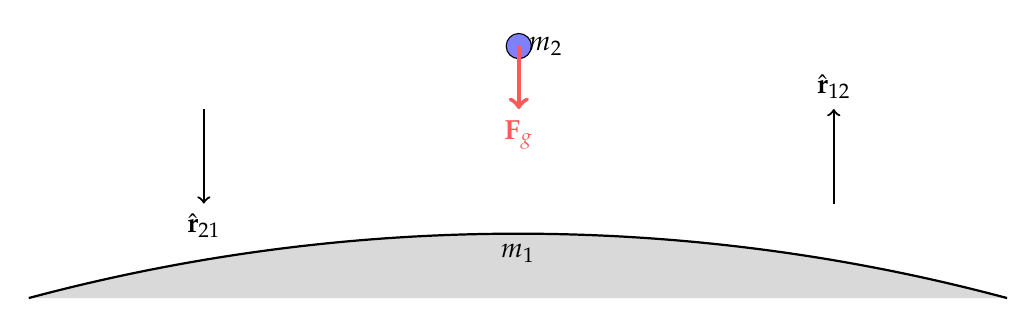
\begin{tikzpicture}[scale=.8]
      \draw[thick,fill=gray!30] (7.75,0) arc(75:105:30)
      node[midway,below]{$m_1$};
      \draw[fill=blue!50] (0,4) circle(.2) node[right]{$m_2$};
      \draw[ultra thick, red!65,->] (0,4)--(0,3)
      node[pos=1,below]{$\mb{F}_g$};
      \draw[->,thick](5,1.5)--(5,3) node[pos=1,above]{$\hat{\mb{r}}_{12}$};
      \draw[->,thick](-5,3)--(-5,1.5) node[pos=1,below]{$\hat{\mb{r}}_{21}$};
    \end{tikzpicture}
  \end{center}

  \eq{-.4in}{
    \boxed{
      \mb{F}_g
      =-\frac{Gm_1m_2}{r^2}\hat{\mb{r}}_{12}
      =+\frac{Gm_1m_2}{r^2}\hat{\mb{r}}_{21}
    }
  }

  where \fbox{$G=\SI{6.67e-11}{N.m^2/kg^2}$} is the universal gravitation
  constant, and $\hat{\mb{r}}_{12}$ and $\hat{\mb{r}}_{21}$ are
  \emph{unit vectors} (length=$1$)
\end{frame}


\begin{frame}
  \frametitle{Universal Gravitation}
  \begin{itemize}
  \item If $m_1$ exerts a gravitational force $\mb{F}_g$ on $m_2$, then $m_2$
    also exerts $-\mb{F}_g$ on $m_1$.
  \item The two forces are equal in magnitude and opposite in direction
    (Newton's 3rd law)
  \item Assumption: $m_1$ and $m_2$ are \emph{point masses}
    that do not occupy any space.
  \item Recall: forces acting on an ensemble of masses is the same as acting at
    its center of mass
  \item Therefore, for the universal gravitational equation to work:
    
    \eq{-.2in}{
      r>(r_1+r_2)
    }
    That is, the two objects hasn't collided into one another
  \end{itemize}
\end{frame}


\section{Gravitational Field}


\begin{frame}
  \frametitle{Think Gravitational Field: What is $g$?}

  We generally describe the force of gravity as
  
  \eq{-.25in}{
    \mb{F}_g=m\mb{g}
  }

  \vspace{-.2in}To find the magnitude of $g$, we group the variables in Newton's
  universal gravitation equation:
    
  \eq{-.2in}{
    F_g=\underbrace{\left[\frac{Gm_1}{r^2}\right]}_{=g}m_2=m_2g
  }

  \vspace{-.1in}On the surface of Earth, we use use $m_1=m_\mathrm{Earth}$ and
  $r=r_\mathrm{Earth}$ to compute $g\approx\SI{10}{m/s^2}$, or
  $g\approx\SI{10}{N/kg}$ (both units are equivalent)
\end{frame}

\begin{frame}
  \frametitle{Gravitational Field}
  The \textbf{gravitational field} $\mb{g}$ generated by a source mass $m_s$
  shows how it influences the gravitational forces on other masses. Its
  \emph{intensity} (i.e.\ magnitude) is defined by:

  \eq{-.25in}{
    \boxed{g(m_s,r)=\frac{Gm_s}{r^2}}
  }
  \begin{center}
    \begin{tabular}{l|c|l}
      \rowcolor{pink}
      \textbf{Quantity} & \textbf{Symbol} & \textbf{SI Unit} \\ \hline
      Gravitational field intensity & $g$ & \si{\newton\per\kilo\gram}
      (newtons per kilogram)\\
      Universal gravitational constant & $G$ &
      \si{\newton\metre^2/\kilo\gram^2} \\
      Mass of source (a point mass) & $m_s$ & \si{\kilo\gram} (kilograms) \\
      Distance from source mass     & $r$ & \si{\metre} (meters)
    \end{tabular}
  \end{center}

  The \emph{direction} of the gravitational field is toward $m_s$.
\end{frame}


\begin{frame}
  \frametitle{Relating Gravitational Field \& Gravitational Force}

  $\mb{g}$ itself doesn't \emph{do} anything until there is another mass $m$. At
  which point, $m$ experiences a gravitational force due to $m_s$, and it is
  related to $\mb{g}$ by:

  \eq{-.2in}{
    \boxed{\mb{F}=m\mb{g}}
  }
  
  $\mb{F}_g$ and  $\mb{g}$ are vectors in the same direction: toward the
  center of the source mass.

  \begin{center}
    \begin{tabular}{l|c|c}
      \rowcolor{pink}
      \textbf{Quantity} & \textbf{Symbol} & \textbf{SI Unit} \\ \hline
      Gravitational field & $\mb{g}$   & \si{N/kg}\\
      Gravitational force on a mass & $\mb{F}_g$ & \si{N} \\
      Mass inside the gravitational field & $m$ & \si{kg} \\
    \end{tabular}
  \end{center}
\end{frame}



\begin{frame}
  \frametitle{What If You Are Inside Another Mass?}
  \framesubtitle{Case 1: A Spherical Shell of Radius $R$}

  \begin{columns}
    \column{.3\textwidth}

    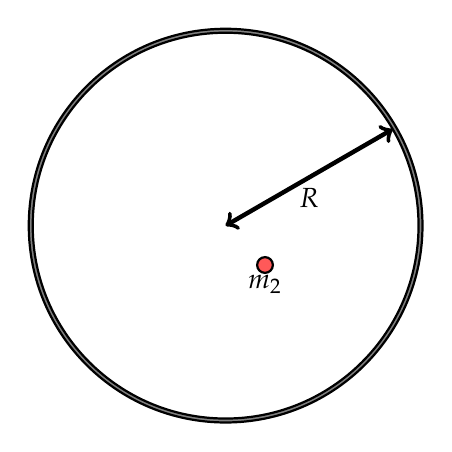
\begin{tikzpicture}[scale=.5]
      \draw[thick,fill=gray](0,0) circle(5);% node[above]{$m_1$};
      \draw[thick,fill=white](0,0) circle(4.9);% node[above]{$m_1$};
      \draw[ultra thick,<->,rotate=30](0,0)--(4.9,0) node[midway,below]{$R$};
      \draw[thick,fill=red!65](1,-1) circle(.2) node[below]{$m_2$};
    \end{tikzpicture}

    \column{.7\textwidth}
    \begin{itemize}
    \item If a mass $m_2$ is \emph{inside} a spherical shell of mass $m_1$, the
      force of gravity it experiences is \textbf{zero}!
      
      \eq{-.3in}{
        \boxed{
          \mb{F}_g=
          \begin{cases}
            \mb{0} & \text{if}\;\;r<R\\
            Gm_1m_2/r^2\hat{\mb{r}} & \text{otherwise}
          \end{cases}
        }
      }
      
    \item\vspace{-.2in} It also means that gravitational field is also
      \textbf{zero}
    \item This is very similar to a charged conducting sphere, where the
      electric field inside is zero.
    \end{itemize}
  \end{columns}
\end{frame}



\begin{frame}
  \frametitle{What If You Are Inside Another Mass?}
  \framesubtitle{Case 2: Uniform Mass of Radius $R$}
  \begin{columns}
    \column{.35\textwidth}

    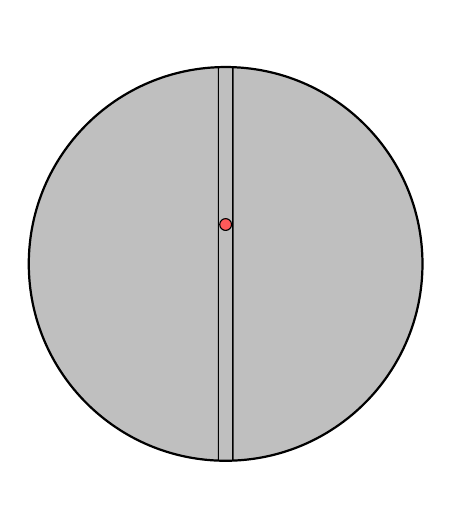
\begin{tikzpicture}[scale=.5]
      \draw[thick,fill=gray!50](0,0) circle(5);
      \clip(-.2,-6) rectangle (.2,6);
      \draw[very thick](.2,5)--(.2,-5);
      \draw[very thick](-.2,5)--(-.2,-5);
      \draw[fill=red!65](0,1) circle(.15) node[right]{$m_2$};
    \end{tikzpicture}

    \column{.65\textwidth}
    Suppose you could drill a hole through the Earth and then drop into
    it. How long would it take you to pop up on the other side of the
    Earth?
  \end{columns}
\end{frame}


\begin{frame}
  \frametitle{Falling To the Center of the Earth}
  Initial gravitational force on the surface is:

  \eq{-.2in}{
    F_g=mg_\mathrm{surface}\quad\quad\quad g_\mathrm{surface}\approx\SI{10}{N/kg}
  }

  \vspace{-.1in}$F_g$ becomes smaller as you approached the center, and when
  you reach the center, $F_g=0$.
  
  \vspace{.1in}Assume that the Earth is uniform density, and neglect air
  resistance and other factors. The value of $g$ as the person falls through
  Earth ($r<R$) is given by:

  \eq{-.3in}{
    g(r)=\frac{GM(r)}{r^2}\quad M(r)=\frac{4}{3}\rho\pi r^3\quad
    \rho=\frac{3M_\mathrm{Earth}}{4\pi R^3}
  }
\end{frame}



\begin{frame}
  \frametitle{Falling To the Center of the Earth}

  \begin{columns}
    \column{.25\textwidth}
    \pic{1.2}{eartholeg.png}

    \column{.75\textwidth}
    Now we have an expression for the gravitational field strength inside
    ``Earth'':

    \eq{-.2in}{
      g(r)=\frac{GM_\mathrm{Earth}r}{R^3}=g_\mathrm{surface}\frac{r}{R}
    }
    
    Gravitational field strength decreases linearly with $r$. At
    the center ($r=0$), $g=0$. Here's the interesting part, the gravitational
    force inside Earth is
    
    \eq{-.2in}{
      F_g=-mg(r)=
      -\underbrace{\left[\frac{mg_\mathrm{surface}}{R}\right]}_{\textrm{constant}} r
      =-kr
    }
  \end{columns}
\end{frame}




\begin{frame}
  \frametitle{Falling To the Center of the Earth}

  \begin{columns}
    \column{.25\textwidth}
    \pic{1}{eartholsat.png}

    \column{.75\textwidth}
    So this poor guy is going to oscillate through Earth with a harmonic motion
    with a period of:

    \eq{-.2in}{
      T=2\pi\sqrt{\frac{m}{k}}
    }

    For Earth, $T=\SI{5068}{\second}$. He would pop up on the opposite side
    after about \SI{42}{min}.

    \vspace{.1in}Suppose a satellite is in a circular orbit just above the
    surface, and passes overhead just above the traveler as he popped up
    out of the hole. The period of such an orbit would be the same as
    oscillating traveler.
    
  \end{columns}
\end{frame}


\begin{frame}
  \frametitle{Gravitational Field Lines}
  \begin{center}
    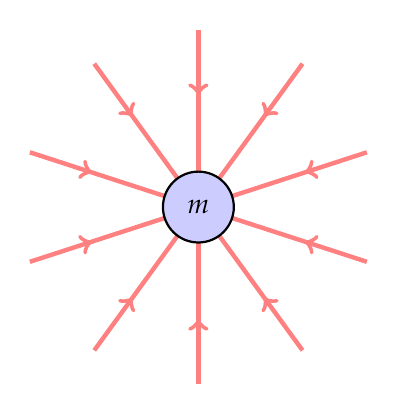
\begin{tikzpicture}[scale=1.5]
      \foreach \x in {0,...,9}\draw[red!50,ultra thick,rotate=36*\x](0,0)--(0,1);
      \foreach \x in {0,...,9}\draw[red!50,<-,ultra thick,rotate around={36*\x:(0,0)}](0,.95)--(0,1.5);
      \draw[fill=blue!20,thick](0,0) circle(.3) node{$m$};
    \end{tikzpicture}
  \end{center}
  \begin{itemize}
  \item The direction of $\mb{g}$ is toward the center of the object that
    created it
  \item Field lines do not tell the intensity (i.e.\ magnitude) of $\mb{g}$,
    only the direction
  \end{itemize}
\end{frame}




\section{Gravitational Potential Energy}


\begin{frame}
  \frametitle{Gravitational Potential Energy}
  \textbf{Gravitational potential energy} is found by integrating the work
  equation and using universal gravitation:

  \vspace{-.25in}{\Large
    \begin{align*}
      W&=\int \mb{F}_g\cdot d\mb{r}=
      -\int_{r_1}^{r_2}\frac{Gm_1m_2}{r^2}\mb{\hat{r}}\cdot d\mb{r}\\
      &=-\int_{r_1}^{r_2}\frac{Gm_1m_2}{r^2}dr=\frac{Gm_1m_2}{r}\Big|^{r_2}_{r_1}
      =-\Delta U_g
    \end{align*}
  }

  \vspace{-.1in}where
  
  \eq{-.35in}{
    \boxed{U_g=-\frac{Gm_1m_2}{r}}
  }
  \begin{itemize}
  \item $U_g$ is the work required to move two objects from $r$ to $\infty$
  \item $U_g=0$ at $r=\infty$ and \emph{decrease} as $r$ decreases
  \end{itemize}
\end{frame}


\begin{frame}
  \frametitle{Relating Gravitational Potential Energy to Force}

  Vector calculus (actually fundamental theorem of calculus) shows that
  gravitational force ($\mb{F}_g$) is the negative gradient of the
  gravitational potential energy ($U_g$):
  
  \eq{-.1in}{
    \mb{F}_g=-\nabla U_g=
    -\frac{\partial U_g}{\partial r}\hat{\mb{r}}
  }

  The direction of $\mb{F}_g$ is always from high to low potential energy
  \begin{itemize}
  \item A falling object is always decreasing in $U_g$
  \item ``Steepest descent'': the direction of $\mb{F}$ is the shortest path
    to decrease $U_g$ 
  \item Objects traveling perpendicular to $\mb{F}_g$ has constant $U_g$
  \end{itemize}
\end{frame}


\begin{frame}
  \frametitle{Relating $U_g$, $\mb{F}_g$ and $\mb{g}$}
  Knowing that $\mb{F}_g$ and $\mb{g}$ only differ by a constant, we can
  also relate gravitational field to $U_g$ by the gradient operator:

  \eq{-.1in}{
    \mb{g}=\frac{\mb{F}_g}{m}=-\nabla\left(\frac{U_g}{m}\right)=
    -\frac{\partial}{\partial r}\left(\frac{U_g}{m}\right)
    \hat{\mb{r}}
  }

  We already know that the direction of $\mb{g}$ is the same as $\mb{F}_g$,
  i.e.
  \begin{itemize}
  \item The direction of $\mb{g}$ is the shortest path to decrease $U_g$ 
  \item Objects traveling perpendicular to $\mb{g}$ has constant $U_g$
  \end{itemize}
\end{frame}



\section{Orbits}

%\begin{frame}
%  \frametitle{Orbital Mechanics \& Kepler's Laws of Planetary Motion}
%  In Physics 12, you studied briefly at the orbits of satellites around Earth,
%  or the orbit of Earth and other planets around the Sun.
%  \begin{itemize}
%  \item Used your understanding of centripetal motion and gravity
%  \item Assumed a circular orbit
%  \end{itemize}
%  Let's review some of those ideas.
%\end{frame}


\begin{frame}
  \frametitle{Orbital Speed}
  \framesubtitle{Newton's Thought Experiment}
  Newton theorized that if the initial velocity of the cannonball is fast
  enough, it will never fall down. So how fast is fast enough?
  \begin{center}
    \pic{.8}{figure-5.jpg}
  \end{center}
  And how fast is too fast that it never comes back?
\end{frame}


\begin{frame}
  \frametitle{Orbital Speed}
  \framesubtitle{Relating Gravitational and Centripetal Force}
  Assuming a small mass $m$ in circular orbit around a much larger mass $M$.
  The required centripetal force is supplied by the gravitational force:
  
  \eq{-.2in}{
    F_g=F_c\quad\longrightarrow\quad \frac{GMm}{r^2}=\frac{mv^2}{r}
  }

  \vspace{-.1in}Solving for $v$, we get the \textbf{orbital speed}
  $v_\mathrm{orbit}$ (aka \textbf{orbital velocity}), which does not depend on
  the mass of the small object in orbit:

  \eq{-.15in}{
    \boxed{v_\mathrm{orbit}=\sqrt{\frac{GM}{r}}}
  }
\end{frame}


%\begin{frame}{Orbital Speed}
%  \framesubtitle{Assumptions vs.\ Reality}
%  \eq{.0in}{
%    \boxed{v_\mathrm{orbit}=\sqrt{\frac{GM}{r}}}
%  }
%  Assumptions:
%  \begin{itemize}
%  \item The orbit of the $m$ must be perfectly circular
%  \item That $M\gg m$, and $M$ can therefore be treated as a fixed point
%  \end{itemize}
%  Reality:
%  \begin{itemize}
%  \item As $m$ is subjected to a centripetal force supplied by the gravity from
%    $M$,\\
%    $M$ is also subjected to a centripetal force supplied by the gravity from
%    $m$.
%  \item $m$ does not actually orbit about the center of $M$, but rather, the
%    center of mass between $M$ and $m$.
%  \end{itemize}
%\end{frame}

\begin{frame}{Escape Speed}
  An object can leave the surface of Earth at any speed. But when all the
  kinetic energy of that object is converted to gravitational potential energy,
  it will return back to the surface of the earth. There is, however, a
  \emph{minimum} velocity at which the object \emph{would not} fall back to
  Earth.
\end{frame}


\begin{frame}
  \frametitle{Escape Speed}
  \begin{itemize}
  \item The gravitational potential energy of an object with mass $m$ on the
    surface of a planet (with mass $M$ and radius $r$) is

    \eq{-.15in}{
      U_g=-\frac{GMm}{r}
    }
  \item The most amount of work that you can do is to bring it to the other side
    of the universe $r=\infty$, where $U_g=0$.
  \item The work by gravity converts kinetic energy into gravitational
    potential energy.
  \item If you start with \emph{more} kinetic energy than required to do all
    the work, then the object has \emph{escaped} the gravitational pull of the
    planet.
  \end{itemize}
\end{frame}


\begin{frame}
  \frametitle{Escape Speed from Circular Orbits}

  Set $K$ to equal to $-U_g$:

  \eq{-.2in}{
    \frac{1}{2}mv^2=\frac{GMm}{r}
  }

  We can then solve for \textbf{escape speed} $v=v_\mathrm{esc}$ (or
  \textbf{escape velocity}):

  \eq{-.2in}{
    \boxed{v_\mathrm{esc}=\sqrt{\frac{2GM}{r}}}
  }

  There is a simple relationship between orbital speed and escape speed:

  \eq{-.2in}{
    \boxed{v_\mathrm{esc}=\sqrt{2} v_\mathrm{orbit}}
  }
\end{frame}



\begin{frame}
  \frametitle{Example Problem}
  \textbf{Example:} Determine the escape velocity and energy for a
  \SI{1.60e4}{\kilo\gram} rocket leaving the surface of Earth.


  \uncover<2>{
    \vspace{.5in}Note: The equation for the escape speed is based on the object
    have a \emph{constant} mass, which is \emph{not} the case for a rocket
    going into space.
  }
\end{frame}


\begin{frame}{What if I'm not escaping from the surface?}
  Both objects have the same escape velocity:
  \begin{center}
    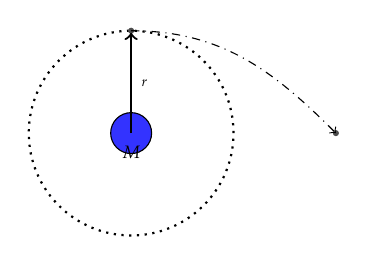
\begin{tikzpicture}[scale=1.3]
      \draw[fill=blue!80](0,0) circle(0.2) node[midway,below]{\tiny $M$};
      \draw[dotted,thick] (0,0) circle(1);
      \fill[black!70](0,1) circle(.03);
      \draw[->,thick](0,0)--(0,.98) node[midway,right]{\tiny $r$};
      \fill[black!70](2,0) circle(.03);
      \draw[->,dash dot](0,1) to[out=0,in=135](2,0);
    \end{tikzpicture}
    \hspace{.3in}
    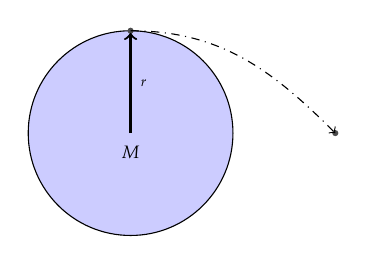
\begin{tikzpicture}[scale=1.3]
      \draw[fill=blue!20] (0,0) circle(1) node[midway,below]{\tiny $M$};
      \fill[black!70](0,1) circle(0.03);
      \draw[->,thick](0,0)--(0,.98) node[midway,right]{\tiny $r$};
      \fill[black!70](2,0) circle(0.03);
        \draw[->,dash dot](0,1) to[out=0,in=135](2,0);      
    \end{tikzpicture}
  \end{center}  
  %Both objects are escaping from distance $r$ from the center of the planet.
  The difference is that the object in orbit (left) already has
  orbital speed $v_\mathrm{orbit}$, so escaping from that orbit requires only an
  additional speed of

    \vspace{-.2in}{\Large
      \begin{displaymath}
        \Delta v=v_\mathrm{esc}-v_\mathrm{orbit}=(\sqrt{2}-1)v_\mathrm{orbit}
      \end{displaymath}
    }
  
\end{frame}


\begin{frame}{What If?}
  What if an object is in an orbit with a speed
  $v_\mathrm{orbit}<v<v_\mathrm{esc}$?

  \vspace{.3in}What if an object has a speed $v<v_\mathrm{orbit}$?
\end{frame}


\begin{frame}{Orbital Energies}
  We can obtain the \textbf{orbital kinetic energy} by using the orbital speed
  in our expression of kinetic energy:

  \eq{-.35in}{
    K_\mathrm{orbit}=\frac{1}{2}mv_\mathrm{orbit}^2=\frac{1}{2}m
    \left(\sqrt{\frac{GM}{r}}\right)^2=\boxed{\frac{GMm}{2r}}
  }

  \vspace{-.11in}We already have an expression for
  \textbf{gravitational potential energy}:

  \eq{-.15in}{
    U_g=-\frac{GMm}{r}=-2K_\mathrm{orbit}
  }
  
  \vspace{-.1in}The \textbf{total orbital energy} is the sum of $K$ and $U_g$:

  \eq{-.15in}{
    E_T=K_\mathrm{orbit}+U_g=-\frac{GMm}{2r}=-K_\mathrm{orbit}
  }
\end{frame}





\section{Orbital Mechanics}


\begin{frame}{Houston, We Have a Problem!}
  As always, this understanding isn't completely correct!
  \begin{itemize}
  \item Centripetal motion is based on rotation around a fixed point, but this
    is \emph{not} the case for orbital mechanics!
  \item Just as Earth experiences a gravitational force by the Sun, the Sun
    also experiences a gravitational force from Earth
  \item The smaller mass $m$ does not actually orbit about the center of the
    larger mass $M$, but rather, the center of mass between $M$ and $m$.
  \item This problem is especially important when the two objects orbiting each
    other has similar masses (e.g.\ a binary star system)
  \end{itemize}
\end{frame}

\begin{frame}{A Central Force}
  Gravity is called a \textbf{central force} in that
  \begin{itemize}
  \item Gravitational force $\mb{F}_g$ is always in the $-\hat{\mb{r}}$
    direction, i.e.\ $\mb{F}\times\mb{r}=\mb{0}$
  \item Therefore gravity doesn't generate any torque
  \item And therefore angular momentum $\mb{L}$ is constant
  \item True regardless of whether the orbit is circular or elliptical
  \end{itemize}
\end{frame}


\begin{frame}{Kepler's Laws of Planetary Motion}
  \begin{enumerate}
  \item\textbf{Law of ellipses:} The orbit of a planet is an ellipse with the
    Sun at one of the two foci.
  \item\textbf{Law of equal areas:} A line segment joining a planet and the Sun
    sweeps out equal areas during equal intervals of time
  \item \textbf{Law of periods:} The square of the orbital period of a planet
    is proportional to the cube of the semi-major axis of its orbit.
  \end{enumerate}

  \vspace{.3in}Johannes Kepler (1571--1630) formulated these laws between 1609
  to 1619 based on interpreting planetary motion data from his teacher, Tycho
  Brahe. It is an improvement over the heliocentric theory of Nicolaus
  Copernicus.
\end{frame}


\begin{frame}
  \frametitle{Kepler's Law of Planetary Motion}
  To fully understand Kepler's laws, we have to first understand the ellipse,
  at least a little bit.

  \begin{columns}
    \column{.3\textwidth}
    \begin{center}
      \pic{1.25}{elliporb.png}
      
      $r' + r =2a$
    \end{center}

    \column{.7\textwidth}
    \begin{itemize}
    \item The area of the ellipse is $A=\pi ab$
    \item For an ellipse, the relationship between $r$ and $\theta$ given by:

      \eq{-.35in}{
        r=\frac{a(1-e^2)}{1+e\cos\theta}
        \quad\textnormal{\normalsize where}\quad
        0\leq e < 1
      }
    \item when $e=0$ it's a circle: $r=a$
    \item When $e=1$ it's no longer an ellipse
    \end{itemize}
  \end{columns}
\end{frame}


\begin{frame}
  \frametitle{Kepler's Law of Planetary Motion}
  \begin{columns}
    \column{.6\textwidth}
    Most of the planets have very small eccentricity, so their orbits are
    fairly close to being circular, but comets are much more eccentric
    \begin{center}
      \pic{.7}{kep5.png}
    \end{center}
    
    \column{.4\textwidth}
    \begin{tabular}{l|l}
      \rowcolor{pink}
      \textbf{Object} & $e$ \\ \hline
      Mercury	& \num{.206} \\
      Venus	& \num{.0068} \\
      Earth	& \num{.0167} \\
      Mars	& \num{.0934} \\
      Jupiter	& \num{.0485} \\
      Saturn	& \num{.0556} \\
      Uranus	& \num{.0472} \\
      Neptune	& \num{.0086} \\
      Pluto	& \num{.25} \\ \hline
      Halley's Comet   & \num{.9671} \\
      Comet Hale-Bopp  & \num{.9951} \\
      Comet Ikeya-Seki & \num{.9999}
    \end{tabular}
  \end{columns}
\end{frame}

\begin{frame}{Reduced Mass}
  When two objects are orbiting each other, the center of mass of the system is
  along the line between them:
  \begin{center}
    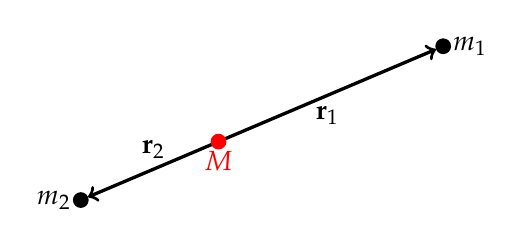
\begin{tikzpicture}
      \begin{scope}[rotate=23]
        \draw[very thick,->](0,0)--(3,0) node[midway,below]{$\mb{r}_1$};
        \draw[very thick,->](0,0)--(-1.8,0) node[midway,above]{$\mb{r}_2$};
        \fill[black] (3.1,0) circle(.1) node[right]{$m_1$};
        \fill[black] (-1.9,0) circle(.1) node[left]{$m_2$};
        \fill[red] (0,0) circle(.1) node[below]{$M$};
      \end{scope}
    \end{tikzpicture}
  \end{center}

  \vspace{-.1in}The vectors $\mb{r}_1$ and $\mb{r}_2$ are relative to the
  center of mass, and the relative position $\mb{r}$ velocity $\mb{v}$ and
  acceleration $\mb{a}$ between $m_1$ and $m_2$ are therefore:
  
  \eq{-.2in}{
    \mb{r}=\mb{r}_2 - \mb{r}_1\quad
    \mb{v}=\mb{v}_2 - \mb{v}_1\quad
    \mb{a}=\mb{a}_2 - \mb{a}_1
  }
\end{frame}



\begin{frame}
  \frametitle{Reduced Mass}
  
  From Newton's third law, we know that the gravitational force exerted by
  $m_1$ on $m_2$ is opposite the force exerted by $m_2$ on $m_1$:

  \eq{-.2in}{
    m_1\mb{a}_1+m_2\mb{a}_2=0
  }

  \vspace{-.2in}Substituting the expression for relative acceleration, we have:

  \eq{-.2in}{
    \mb{a}=\mb{F}_g\left[\frac{1}{m_1}+\frac{1}{m_2}\right]=
    \mb{F}_g\left[\frac{m_1+m_2}{m_1m_2}\right]=\frac{\mb{F}_g}{\mu}
  }
  
  We can now define a new concept called \textbf{reduced mass}:
  
  \eq{-.2in}{
    \mu=\frac{m_1m_2}{m_1+m_2}
  }
\end{frame}


\begin{frame}
  \frametitle{An Equivalent System}
  The orbit of one of the masses in a binary system is equivalent to the motion
  of the reduced mass orbiting around a point at relative distance $r$ where
  the total mass $M$ is placed. The magnitude of $r$ is the same as the
  relative distance $r$ in the development above.
  \begin{center}
    \vspace{-.2in}
    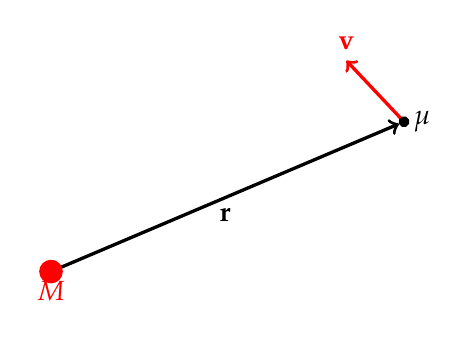
\begin{tikzpicture}
      \begin{scope}[rotate=23]
        \draw[very thick,->](0,0)--(4.8,0) node[midway,below]{$\mb{r}$};
        \draw[very thick,->,red](4.87,0)--(4.5,1) node[pos=1,above]{$\mb{v}$};
        \fill[red] (0,0) circle(.15) node[below]{$M$};
        \fill[black] (4.87,0) circle(.07) node[right]{$\mu$};
      \end{scope}
    \end{tikzpicture}
  \end{center}
\end{frame}


\begin{frame}{Kepler's First Law}
  \begin{columns}
    \column{.3\textwidth}
    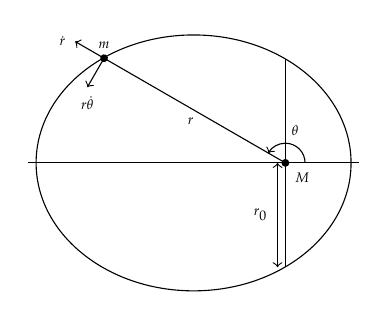
\begin{tikzpicture}[scale=.5]
      \def\a{4} % semi-major axis
      \def\b{3.25} % semi-minor axis
      \def\angle{150} % angle
      \draw (0,0) ellipse ({\a} and {\b});% Draw the ellipse
      \draw ({sqrt(\a*\a-\b*\b)},-2.65)--({sqrt(\a*\a-\b*\b)},2.65);
      \draw (-\a-.2,0)--(\a+.2,0);
      \fill[black]({sqrt(\a*\a-\b*\b)},0) circle(.1)
      node[below right]{\tiny $M$};
      \begin{scope}[rotate around={\angle:({sqrt(\a*\a-\b*\b)},0)}]
        \draw[->]({sqrt(\a*\a-\b*\b)},0)--(8.5,0)
        node[pos=.45,below]{\tiny$r$}
        node[pos=1,left]{\tiny $\dot{r}$};
        \draw[->](7.65,0)--(7.65,.85) node[below]{\tiny $r\dot{\theta}$};
        \fill (7.65,0) circle(.1) node[above]{\tiny $m$};
      \end{scope}
      \draw[->]({sqrt(\a*\a-\b*\b)+.5},0) arc(0:\angle:.5)
      node[pos=.4,above]{\tiny$\theta$};
      \draw[<->]({sqrt(\a*\a-\b*\b)-.2},0)--({sqrt(\a*\a-\b*\b)-.2},-2.65)
      node[midway,left]{\tiny$r_0$};
    \end{tikzpicture}
    \column{.7\textwidth}
    The total energy of the object $m$ (reduced mass) in orbit around $M$
    (total mass):

    \vspace{-.35in}{\Large
      \begin{align*}
        E_T&=K +U_g=\frac{1}{2}mv^2-\frac{GMm}{r^2}\\
        &=\frac{1}{2}m(\dot{r}^2+r^2\dot{\theta}^2)-\frac{GMm}{r^2}
      \end{align*}
    }
    \begin{itemize}
    \item\vspace{-.1in}$v_r=\dot{r}=dr/dt$ is the radial component of velocity
    \item $v_\theta=r\omega=r\dot{\theta}$ is the angular component
    \item The two velocity components are orthogonal $\therefore$
      $v^2=v_r^2+v_\theta^2$
    \end{itemize}
  \end{columns}
\end{frame}




\begin{frame}{Kepler's First Law}
  \begin{columns}
    \column{.3\textwidth}
    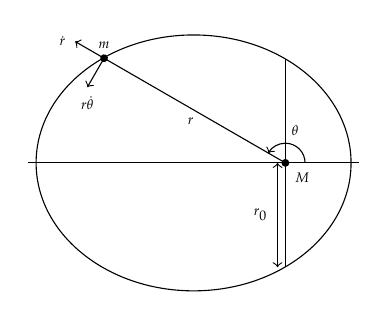
\begin{tikzpicture}[scale=.5]
      \def\a{4} % semi-major axis
      \def\b{3.25} % semi-minor axis
      \def\angle{150} % angle
      \draw (0,0) ellipse ({\a} and {\b});% Draw the ellipse
      \draw ({sqrt(\a*\a-\b*\b)},-2.65)--({sqrt(\a*\a-\b*\b)},2.65);
      \draw (-\a-.2,0)--(\a+.2,0);
      \fill[black]({sqrt(\a*\a-\b*\b)},0) circle(.1)
      node[below right]{\tiny $M$};
      \begin{scope}[rotate around={\angle:({sqrt(\a*\a-\b*\b)},0)}]
        \draw[->]({sqrt(\a*\a-\b*\b)},0)--(8.5,0)
        node[pos=.45,below]{\tiny$r$}
        node[pos=1,left]{\tiny $\dot{r}$};
        \draw[->](7.65,0)--(7.65,.85) node[below]{\tiny $r\dot{\theta}$};
        \fill (7.65,0) circle(.1) node[above]{\tiny $m$};
      \end{scope}
      \draw[->]({sqrt(\a*\a-\b*\b)+.5},0) arc(0:\angle:.5)
      node[pos=.4,above]{\tiny$\theta$};
      \draw[<->]({sqrt(\a*\a-\b*\b)-.2},0)--({sqrt(\a*\a-\b*\b)-.2},-2.65)
      node[midway,left]{\tiny$r_0$};
    \end{tikzpicture}

    \column{.7\textwidth}
    The angular momentum (a constant!) of $m$ about $M$ is:

    \eq{-.2in}{
      L=mr^2\dot{\theta}\;\;\rightarrow\;\;\dot{\theta}=\frac{L}{mr^2}
    }

    \vspace{-.1in}We make a subsitution of $\rho=1/r$, and then integrating with
    time:

    \eq{-.25in}{
      \theta=\int\frac{L}{m}\rho^2dt=\int\frac{L}{m}\rho^2\frac{dt}{d\rho}d\rho
    }

    \vspace{-.1in}But since
    $\dot{r}=\frac{dr}{dt}=\frac{-1}{\rho^2}\frac{d\rho}{dt}$, the integral
    reduces to:

    \eq{-.2in}{\theta=-\int\frac{L}{m\dot{r}}d\rho}    
  \end{columns}
\end{frame}


\begin{frame}{Kepler's First Law}
  \begin{columns}
    \column{.3\textwidth}
    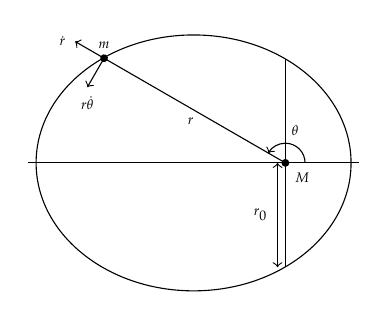
\begin{tikzpicture}[scale=.5]
      \def\a{4} % semi-major axis
      \def\b{3.25} % semi-minor axis
      \def\angle{150} % angle
      \draw (0,0) ellipse ({\a} and {\b});% Draw the ellipse
      \draw ({sqrt(\a*\a-\b*\b)},-2.65)--({sqrt(\a*\a-\b*\b)},2.65);
      \draw (-\a-.2,0)--(\a+.2,0);
      \fill[black]({sqrt(\a*\a-\b*\b)},0) circle(.1)
      node[below right]{\tiny $M$};
      \begin{scope}[rotate around={\angle:({sqrt(\a*\a-\b*\b)},0)}]
        \draw[->]({sqrt(\a*\a-\b*\b)},0)--(8.5,0)
        node[pos=.45,below]{\tiny$r$}
        node[pos=1,left]{\tiny $\dot{r}$};
        \draw[->](7.65,0)--(7.65,.85) node[below]{\tiny $r\dot{\theta}$};
        \fill (7.65,0) circle(.1) node[above]{\tiny $m$};
      \end{scope}
      \draw[->]({sqrt(\a*\a-\b*\b)+.5},0) arc(0:\angle:.5)
      node[pos=.4,above]{\tiny$\theta$};
      \draw[<->]({sqrt(\a*\a-\b*\b)-.2},0)--({sqrt(\a*\a-\b*\b)-.2},-2.65)
      node[midway,left]{\tiny$r_0$};
    \end{tikzpicture}

    \column{.7\textwidth}

    Combining the equations for angular momentum and tatal energy, and solving
    for $\dot{r}$:
    
    \eq{-.25in}{
      \dot{r}^2=\frac{2E}{m}+2GM\rho-\frac{L^2}{m^2}\rho^2
    }

    \vspace{-.1in}Now the crazy manipulation (totally \emph{not} obvious) by
    this substitution (both are constants):

    \vspace{-.37in}{\large
      \begin{align*}
        r_0&=\frac{L^2}{GMm^2}\\
        e^2&=1+\frac{2Er_0}{GMm}
      \end{align*}
    }

    \vspace{-.2in}This way, when we solve for $r$, we have an expression that
    is immediately recognizable as an ellipse.
  \end{columns}
\end{frame}

\begin{frame}{Kepler's First Law}
  After our manipulation, we get (after a bit of algebra):

  \eq{-.25in}{
    \dot{r}
    =\frac{L}{m}
    \left[\frac{e^2}{r_0^2}-\left(\rho-\frac{1}{r_0} \right)\right]^{1/2}
  }
  
  \vspace{-.1in}which we will substitute into the expression for
  $\dot{\theta}$, and get:

  \vspace{-.35in}{\Large
    \begin{align*}
      \theta&=-\int\frac{1}{\sqrt{(e/r_0)^2-(\rho-1/r_0)^2}}d\rho\\
      &=\cos^{-1}\left(\frac{\rho-1/r_0}{e/r_0}\right)
      \end{align*}
  }
\end{frame}


\begin{frame}{Kepler's First Law}
  Most importantly, once we untangle the last equation, we have a simple
  expression of:

  \eq{-.2in}{
    r=\frac{r_0}{1+e\cos\theta}
  }
  
  which is the equation for an ellipse. We can now say that $e$ is the
  eccentricity of the ellipse and $r_0=a(1-e^2)$ is the semi-latus rectum of the
  ellipse.
\end{frame}

%\begin{frame}
%  \frametitle{Now The Complicated Math}
%  To show that the orbit is an ellipse (or it can be an ellipse), we need to
%  show that the relationship between $r$ and $\theta$ is the one
%  that we described earlier:
%
%  \eq{-.15in}{
%    r=\frac{a(1-e^2)}{1+e\cos\theta}
%  } 
%  
%  The following steps will be shown \emph{only once}, and it's not important to
%  be able to follow/remember everything here.
%\end{frame}
%
%
%
%\begin{frame}
%  \frametitle{Complicated Calculations}
%  The acceleration of the reduced mass:
%
%  \eq{-.15in}{
%    \mb{a}=-\frac{GM}{r^2}\hat{\mb{r}}
%  }
%
%  To find the expression for $r$, we do a cross product of $\mb{a}$ with
%  $\mb{L}$:
%  
%  \eq{-.3in}{
%    \mb{a}\times\mb{L}=-\frac{GM}{r^2}\hat{\mb{r}}\times
%    \left(\mu r^2\hat{\mb{r}}\times\frac{d\hat{\mb{r}}}{dt} \right)
%    =GM\mu\hat{\mb{r}}\times
%    \left(\hat{\mb{r}}\times\frac{d\hat{\mb{r}}}{dt} \right)
%  }
%  
%  We then apply the vector identity
%  $\mb{A}\times(\mb{B}\times\mb{C})=(\mb{A}\cdot\mb{C})\mb{B}-(\mb{A}\cdot\mb{B})\mb{C}$ and the expression magically reduces to:
%
%  \eq{-.3in}{
%    \mb{a}\times\mb{L}=GM\mu\frac{d\hat{\mb{r}}}{dt}
%  }
%\end{frame}
%
%
%
%\begin{frame}
%  \frametitle{Confused Yet?}
%  Now we move on to another expression that is closer to where we need to be:
%
%  \eq{-.25in}{
%    \frac{d}{dt}\left(\mb{v}\times\mb{L}\right)=
%    \frac{d\mb{v}}{dt}\times\mb{L} +
%    \mb{v}\times \cancel{\frac{d\mb{L}}{dt}}=\mb{a}\times\mb{L}
%    =\frac{d}{dt}\left(GM\mu\hat{\mb{r}}\right)
%  }
%
%  Integrating both sides with respect to $t$ and we get:
%
%  \eq{-.2in}{
%    \mb{v}\times\mb{L}=GM\mu\hat{\mb{r}} +\mb{D}
%  }
%  where $\mb{D}$ is some constant of integration. Now we take the dot product
%  with $\mb{r}$
%
%  \eq{-.2in}{
%    \mb{r}\cdot\left(\mb{v}\times\mb{L}\right)
%    =GM\mu r + \mb{r}\cdot\mb{D}
%  }
%\end{frame}
%
%
%
%\begin{frame}
%  \frametitle{Just One More Slide!}
%  We once again apply some vector identity:
%  $\mb{A}\cdot(\mb{B}\times\mb{C})=(\mb{A}\times\mb{B})\cdot\mb{C}$ and we
%  get:
%
%  \eq{-.3in}{
%    \left(\mb{r}\times\mb{v}\right)\cdot\mb{L}
%    =GM\mu r + rD\cos\theta
%  }
%
%  \vspace{-.2in}The final step is to recognize that if we define $e=D/GM\mu$,
%  then we can express $r$ as:
%  
%  \eq{-.3in}{
%    r=\frac{L^2/\mu^2}{GM(1+e\cos\theta)}
%  }
%  
%  This is an expression for an ellipse!
%    
%  \eq{-.2in}{
%    r=\frac{a(1-e^2)}{1+e\cos\theta}\quad\textnormal{if}\quad
%    L=\mu\sqrt{GMa(1-e^2)}
%  }  
%\end{frame}
%
%
%\begin{frame}
%  \frametitle{Kepler's First Law: Law of Orbits}
%  \begin{columns}
%    \column{.3\textwidth}
%    \vspace{.2in}\pic{1.2}{kepo17.png}
%    
%    \column{.7\textwidth}
%    \begin{center}
%      \fbox{
%        \begin{minipage}{.85\textwidth}
%          For a bound binary orbit, each object will follow an elliptical orbit
%          about the center of mass of the system. The center of mass will be at
%          one focus of each ellipse
%        \end{minipage}
%      }
%    \end{center}
%    \begin{itemize}
%    \item This is \emph{slightly} different from Kepler's conclusion!
%    \item But if one of the mass is very large compared to the other one,
%      i.e.\ $m_1\gg m_2$, then the center of gravity is essentially at the
%      center of $m_1$ and $m_2$ is orbiting around $m_1$ in an ellipse
%    \end{itemize}
%  \end{columns}
%\end{frame}



\begin{frame}{Kepler's 2nd Law: The Law of Equal Areas}

  \vspace{.2in}
  \begin{center}
    \fbox{
      \begin{minipage}{.9\textwidth}
      \textbf{Second Law: A line segment joining a planet and the Sun sweeps
        out equal areas during equal intervals of time}
      \end{minipage}
    }

    \pic{.6}{201532-132212364-3243-planet.jpg}
  \end{center}
\end{frame}


\begin{frame}
  \frametitle{Kepler's 2nd Law: The Law of Equal Areas}
  \begin{center}
    \fbox{
      \begin{minipage}{.9\textwidth}
      \textbf{Second Law: A line segment joining a planet and the Sun sweeps
        out equal areas during equal intervals of time}
      \end{minipage}
    }
  \end{center}

  \begin{columns}
    \column{.25\textwidth}
    %\pic{1.1}{kepa1.png}
    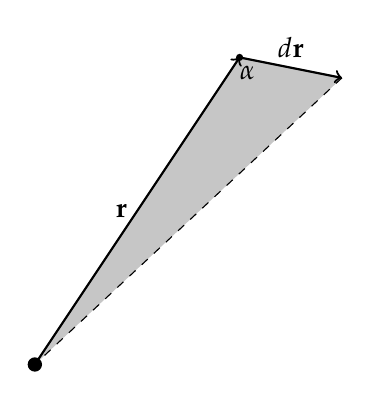
\begin{tikzpicture}[scale=1.3]
      \fill[gray!45](0,0)--(2,3)--(3,2.8)--cycle;
      \draw[->,thick](0,0)--(2,3)
      node[midway,left]{$\mb{r}$} node[pos=.95,right]{$\alpha$};
      \draw[->,thick](2,3)--(3,2.8) node[midway,above]{$d\mb{r}$};
      \draw[dashed](3,2.8)--(0,0);
      \fill[black](0,0) circle(.07);
      \fill[black](2,3) circle(.035);
    \end{tikzpicture}
    \column{.75\textwidth}
    The infinitesimal area swept out by an object in orbit is given by
    
    \eq{-.4in}{
      dA=\frac{1}{2}rdr\sin\alpha
      \;\;\rightarrow\;\;
      d\mb{A}=\frac{1}{2}\mb{r}\times d\mb{r}
    }

    \vspace{-.15in}The time derivative gives an expression for
    \emph{areal velocity} (yes, that's a real word):
      
    \eq{-.35in}{
      \dot{\mb{A}}=\frac{d\mb{A}}{dt}
      =\frac{1}{2}\mb{r}\times\frac{d\mb{r}}{dt}
      =\frac{1}{2}\mb{r}\times\dot{\mb{r}}
      =\frac{1}{2}(\mb{r}\times\mb{v})
    }
    
  \end{columns}
\end{frame}


\begin{frame}{Kepler's Second Law}
  We can express $\mb{r}\times\mb{v}$ in terms of angular momentum,
  $\mb{L}=m(\mb{r}\times\mb{v})$. But in motion under any central force (such
  as gravity), angular momentum is a constant, and therefore:

  \eq{-.2in}{
    \dot{\mb{A}}=\frac{1}{2}(\mb{r}\times\mb{v})=\frac{\mb{L}}{2m}=
    \text{constant}
  }

  As predicted by Kepler's second law.
%  A vector's cross product with itself is zero, i.e.\ $\mb{r}\times\mb{r}=0$.
%  In the second term, $\ddot{\mb{r}}$ is the acceleration due to gravity, which
%  is opposite in direction to $\mb{r}$, so the cross product $
%  \mb{r}\times\ddot{\mb{r}}$ is also zero, and we have
%
%  \eq{-.2in}{
%    \ddot{\mb{A}}=\mb{0}\;\;\rightarrow\;\;\dot{\mb{A}}=\text{constant}
%  }
%
%  \vspace{-.1in}This is true for any motion under a central force.
\end{frame}

%\begin{frame}
%  \frametitle{Kepler's 2nd Law: The Law of Equal Areas}
%
%  But hurray! We know that the angular component of velocity ($\mb{v}_\theta$)
%  is related to the angular velocity $\bm{\omega}$, so:
%    
%  \eq{-.25in}{
%    v_\theta=r\omega\quad\longrightarrow\quad
%    \frac{dA}{dt}
%    =\frac{1}{2}r(r\omega)
%    =\frac{1}{2}rv_\theta
%  }
%
%  Hurray again! Because we know that
%    
%  \eq{-.4in}{
%    rv_\theta
%    =\left|\mb{r}\times\mb{v}_\theta\right|
%    =\left|\frac{\mb{L}}{\mu}\right|=\frac{L}{\mu}
%    \quad\longrightarrow\quad
%    \boxed{\frac{dA}{dt} =\frac{L}{2\mu}}
%  }
%
%  Since we know that angular momentum is conserved (i.e. $L$ is constant),
%  areal velocity is a constant, therefore it sweeps out equal areas in equal
%  intervals of time
%\end{frame}


\begin{frame}
  \frametitle{Kepler's Third Law: The Law of Periods}
  \begin{center}
    \fbox{
      \begin{minipage}{.9\textwidth}
        \textbf{Law of Periods: The square of the orbital period of a planet
          is proportional to the cube of the semi-major axis of its orbit.}
      \end{minipage}
    }

    \vspace{.2in}\pic{.5}{kep8.png}
  \end{center}
\end{frame}


\begin{frame}{Kepler's Third Law: The Law of Periods}

  The area swept by the planet through one orbital period is the areal velocity
  (constant!) integrated by time, from $t=0$ to $t=T$:

  \eq{-.2in}{
    A=\int dA=\int_0^T\frac{dA}{dt}dt=\frac{L}{2m}\int_0^Tdt=\frac{L}{2m}T
  }
  
  From Kepler's first law, this area is an ellipse, given by the equation based
  on $a$ (the semi-major axis), $b$ (the semi-minor axis):

  \eq{-.25in}{
    A=\pi ab=\pi a^2\sqrt{1-e^2}
  }
  \vspace{-.1in}Combining the two equations above give this expression:

  \eq{-.15in}{
    T^2=\frac{m^2}{L^2}4\pi^2a^4(1-e^2)
  }
\end{frame}


\begin{frame}
  \frametitle{Kepler's Third Law: The Law of Periods}

  But we also (from proving the first law) have:

  \eq{-.2in}{
    r_0=a(1-e^2)=\frac{L^2}{GMm^2}
  }

  Substituting this expression into the equation for the period, and after some
  more algebra, we end up with this expression:

  \eq{-.2in}{
    \boxed{T^2
      =\left[\frac{4\pi^2}{GM}\right] a^3
    }
  }

  In cases where $m_2 \ll m_1$ (e.g.\ Earth orbiting the sun),
  $M=m_1+m_2\approx m_1$.
\end{frame}

\end{document}
